\clearpage

\section{Photodiode}

This block simulates a block of two photodiodes assembled like in figure~\ref{photodiode}. It accepts two optical input signals and outputs one electrical signal. Each photodiode converts an optical signal to an electrical signal. The two electrical signals are then subtracted and the resulting signals corresponds to the output signal of the block.

\begin{figure}[h]
	\centering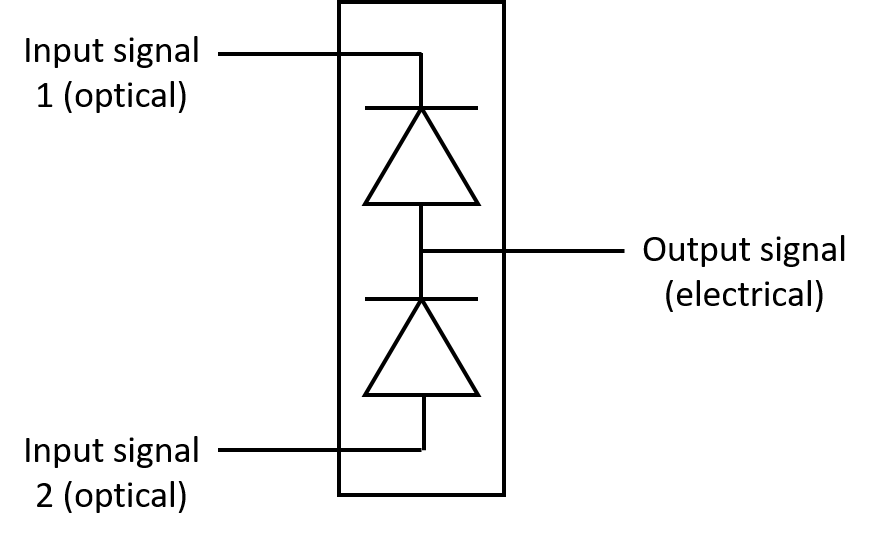
\includegraphics[width=0.5\textwidth]{../homodyne_receiver/figures/photodiode.png}
	\caption{Schematic representation of the physical equivalent of the photodiode code block}\label{photodiode}
\end{figure}

\subsection*{Input Parameters}

\begin{itemize}
	\item responsivity\{1\}
	\item outputOpticalWavelength\{ 1550e-9 \}
	\item outputOpticalFrequency\{ SPEED\_OF\_LIGHT / wavelength \}
\end{itemize}

\subsection*{Methods}
 
Photodiode() {}
\bigbreak
Photodiode(vector$<$Signal *$>$ \&InputSig, vector$<$Signal *$>$ \&OutputSig) :Block(InputSig, OutputSig) {}
\bigbreak
void initialize(void)
\bigbreak
bool runBlock(void)
\bigbreak
void setResponsivity(\texttt{t\_real} Responsivity)

\subsection*{Functional description}

This block accepts two input optical signals. It computes the optical power of the signal (given by the absolute value squared of the input signal) and multiplies it by the \textit{responsivity} of the photodiode. This product corresponds to the current generated by the photodiode. This is done for each of the input signals. The two currents are then subtracted producing a single output current, that corresponds to the output electrical signal of the block.

\pagebreak

\subsection*{Input Signals}

\subparagraph*{Number:} 2

\subparagraph*{Type:} Optical (OpticalSignal)

\subsection*{Output Signals}

\subparagraph*{Number:} 1

\subparagraph*{Type:} Electrical (TimeContinuousAmplitudeContinuousReal)

\subsection*{Examples} 

\begin{figure}[h]
	\centering
	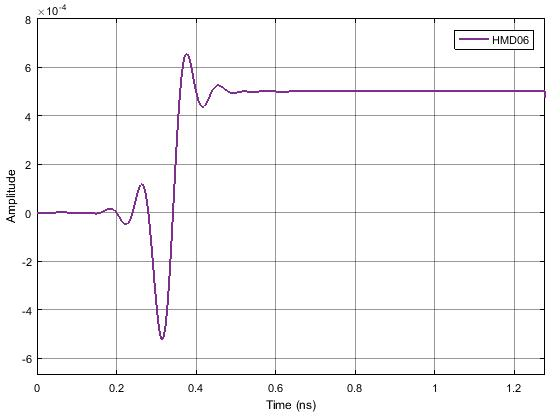
\includegraphics[width=\textwidth]{../homodyne_receiver/figures/Photodiode_output}
	\caption{Example of the output singal of the photodiode block for a bunary sequence 01}\label{Photodiode_output}
\end{figure}

\subsection*{Sugestions for future improvement}

